\documentclass[convert={outfile=mlp_model.png}]{standalone}

% Now include my standard packages, which also includes:
\usepackage{standalone}
\usepackage{tikz}
\usetikzlibrary{positioning}

\tikzstyle{inputNode}=[draw,circle,minimum size=10pt,inner sep=0pt]
\tikzstyle{stateTransition}=[-stealth, thick]

\begin{document}
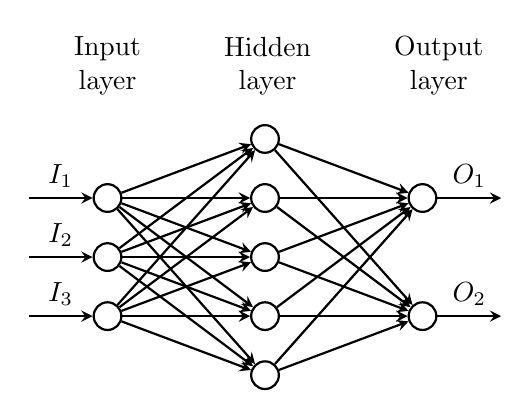
\begin{tikzpicture}
	\node[inputNode, thick] (i1) at (6, 0.75) {};
	\node[inputNode, thick] (i2) at (6, 0) {};
	\node[inputNode, thick] (i3) at (6, -0.75) {};
	
	\node[inputNode, thick] (h1) at (8, 1.5) {};
	\node[inputNode, thick] (h2) at (8, 0.75) {};
	\node[inputNode, thick] (h3) at (8, 0) {};
	\node[inputNode, thick] (h4) at (8, -0.75) {};
	\node[inputNode, thick] (h5) at (8, -1.5) {};
	
	\node[inputNode, thick] (o1) at (10, 0.75) {};
	\node[inputNode, thick] (o2) at (10, -0.75) {};
	
	\draw[stateTransition] (5, 0.75) -- node[above] {$I_1$} (i1);
	\draw[stateTransition] (5, 0) -- node[above] {$I_2$} (i2);
	\draw[stateTransition] (5, -0.75) -- node[above] {$I_3$} (i3);
	
	\draw[stateTransition] (i1) -- (h1);
	\draw[stateTransition] (i1) -- (h2);
	\draw[stateTransition] (i1) -- (h3);
	\draw[stateTransition] (i1) -- (h4);
	\draw[stateTransition] (i1) -- (h5);
	\draw[stateTransition] (i2) -- (h1);
	\draw[stateTransition] (i2) -- (h2);
	\draw[stateTransition] (i2) -- (h3);
	\draw[stateTransition] (i2) -- (h4);
	\draw[stateTransition] (i2) -- (h5);
	\draw[stateTransition] (i3) -- (h1);
	\draw[stateTransition] (i3) -- (h2);
	\draw[stateTransition] (i3) -- (h3);
	\draw[stateTransition] (i3) -- (h4);
	\draw[stateTransition] (i3) -- (h5);
	
	\draw[stateTransition] (h1) -- (o1);
	\draw[stateTransition] (h1) -- (o2);
	\draw[stateTransition] (h2) -- (o1);
	\draw[stateTransition] (h2) -- (o2);
	\draw[stateTransition] (h3) -- (o1);
	\draw[stateTransition] (h3) -- (o2);
	\draw[stateTransition] (h4) -- (o1);
	\draw[stateTransition] (h4) -- (o2);
	\draw[stateTransition] (h5) -- (o1);
	\draw[stateTransition] (h5) -- (o2);
	
	\node[above=of i1, align=center] (l1) {Input \\ layer};
	\node[right=2.3em of l1, align=center] (l2) {Hidden \\ layer};
	\node[right=2.3em of l2, align=center] (l3) {Output \\ layer};
	
	\draw[stateTransition] (o1) -- node[above] {$O_1$} (11, 0.75);
	\draw[stateTransition] (o2) -- node[above] {$O_2$} (11, -0.75);
\end{tikzpicture}
\end{document}